\documentclass[10pt]{article}
\usepackage{tikz}
\usetikzlibrary{arrows.meta, positioning, shadows}

\begin{document}
 Alice was beginning to get very tired of sitting by her sister on the bank, and of having nothing to do: once or twice she had peeped into the book her sister was reading, but it had no pictures or conversations in it, “and what is the use of a book,” thought Alice “without pictures or conversations?”

    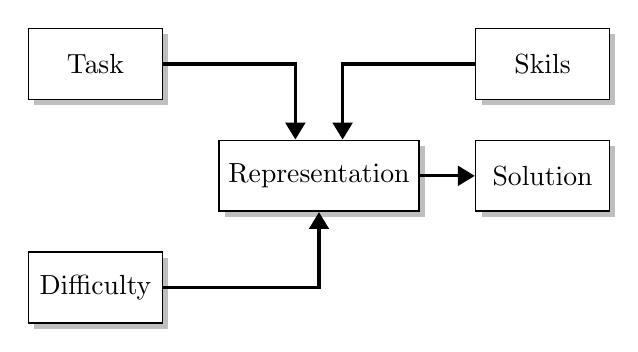
\begin{tikzpicture}[
        node distance = 5mm and 7mm,
           arr/.style = {-Triangle,very thick},
           box/.style = {rectangle, draw, semithick,
                         minimum height=9mm, minimum width=17mm,
                         fill=white, drop shadow},
                                ]
        \node (n1) [box] {Task};
        \node (n2) [box, below right=of n1] {Representation};
        \node (n3) [box, above right=of n2] {Skils};
        \node (n4) [box, below  left=of n2] {Difficulty};
        \node (n5) [box, right=of n2] {Solution};
        %
        \draw[arr]   (n1) -| ([xshift=-3mm] n2.north);
        \draw[arr]   (n3) -| ([xshift= 3mm] n2.north);
        \draw[arr]   (n4) -| (n2);
        \draw[arr]   (n2) -- (n5);
    \end{tikzpicture}
    
    So she was considering in her own mind (as well as she could, for the hot day made her feel very sleepy and stupid), whether the pleasure of making a daisy-chain would be worth the trouble of getting up and picking the daisies, when suddenly a White Rabbit with pink eyes ran close by her. 
\end{document}